\chapter{Foundation}

In vessel handling terminology, maneuvering refers to the task of controlling a vessel’s movement using its propulsion and navigation systems; taking into account environmental forces such as wind, waves and, current acting on the vessel. Vessels move in a variety of marine environments. Starting from ports in harbors where the water is shallow and vessel traffic is high, a vessel might navigate the vast open seas to a different port in a harbour across the ocean. Vessels also navigate inland waterways such as rivers, canals, backwaters and creeks. More recently, developments in offshore wind farming and the oil and gas industry have necessitated regular and frequent visits to offshore structures located on continental shelves. Figure \ref{fig:northseamap} shows some prominent offshore oil fields in the North sea. 

%\begin{figure}
%	\centering
%	\begin{subfigure}{0.4\linewidth}
%		\centering
%		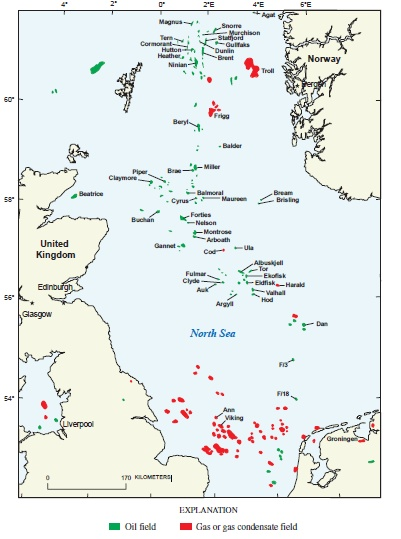
\includegraphics[scale=0.5]{northseaoilandgasmap}
%		\caption{Map of oil and gas fields in the North sea}
%		\label{fig:northseamap}
%	\end{subfigure}
%	\begin{subfigure}{0.4\linewidth}
%		\centering
%		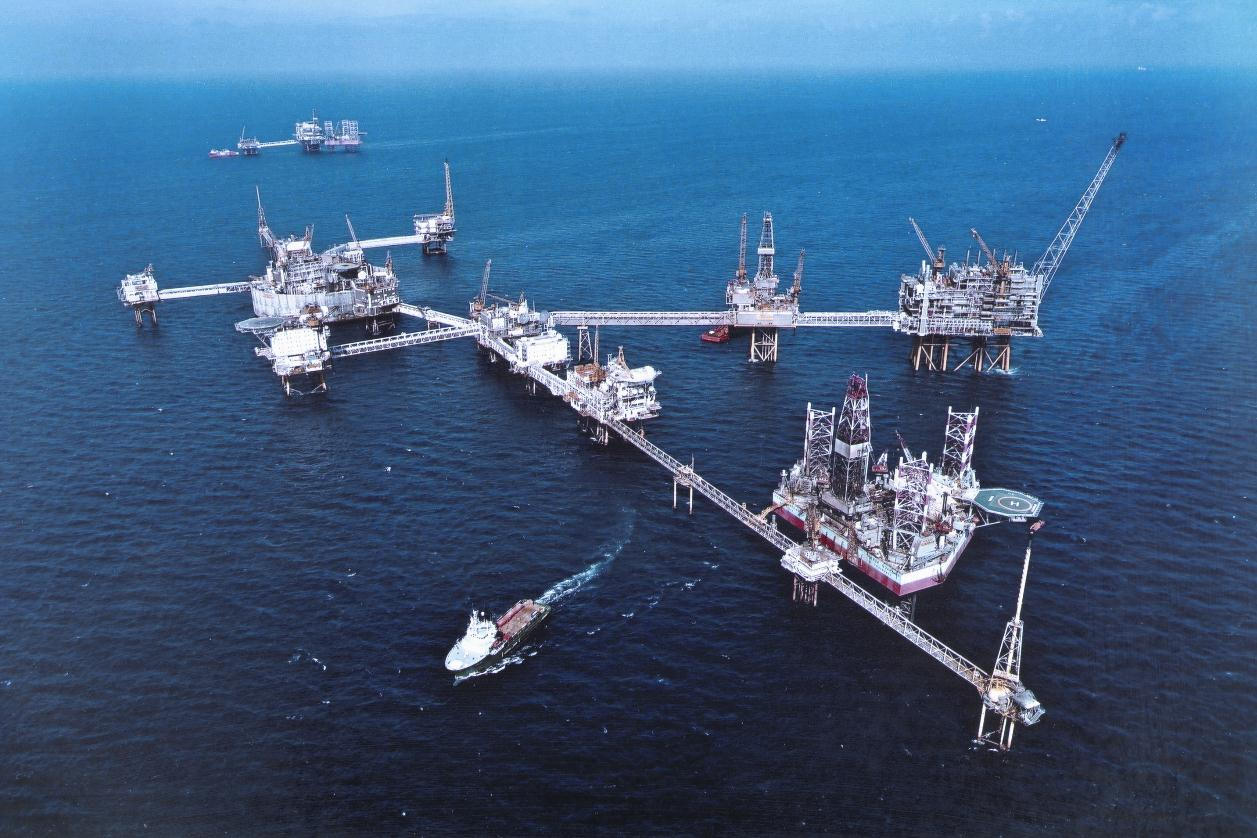
\includegraphics[scale=0.25]{ekofisk}
%		\caption{Ekofisk oil field in the Norwegian sector of the North Sea}
%		\label{fig:ekofisk}
%	\end{subfigure}
%	\caption{Offshore oil and gas fields in the North sea}
%	\label{fig:northseaoilandgas}
%\end{figure}

\begin{figure}
	\centering
	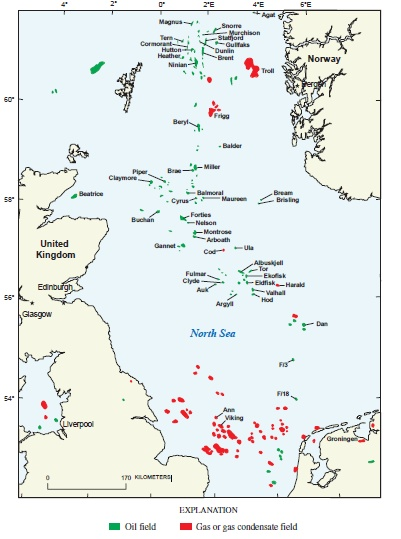
\includegraphics[scale=0.8]{northseaoilandgasmap}
	\caption{Map of oil and gas fields in the North sea}
	\todo[inline]{Get higher resolution picture}
	\label{fig:northseamap}
\end{figure}

% More recently, offshore wind energy and the oil and gas industry have  offshore structures typically located on continental shelves some miles off the coast. 


%Recently, developments in the oil and gas industry have necessitated extensive use of specialised vessels called offshore supply vessels in aid of exploration and production operations. These 

%the construction and maintenance of offshore oil platforms typically located in continental shelves. 

Handling large vessels at low speeds has been difficult on marine vessels historically. The working mechanism of rudder systems of the past made it difficult to turn large vessels in place. From a human operator perspective, the challenge of maneuvering at low speed is further amplified when the operation occurs in close proximity to large physical objects in the vicinity. The stress from risk of collision adds to the difficulty of the task. Refer to \citep{inoue2000evaluation} for a objective evaluation of ship handling difficulties arising from restricted maneuvering area or traffic congestion. Examples of difficult maneuvering operations are approaching a harbour, berthing, sailing side-by-side another vessel, approaching and stationing close to an oil platform, etc. An often recurring sequence is that of  port-bound vessel heading to its berthing location in the harbour. Having entered pilot waters from seaward, its course needs to be controlled to ensure safe passage through channels, bridges, and locks; while avoiding collisions with other vessels at the same time. Safety risks involved in such tasks make it a stressful operation. Mistakes have high associated costs, possibly leading to lost lives and damage to expensive constructions.

% Mistakes in execution have high costs associated with them as they can lead to lost lives and damage to expensive constructions. 

%Executing a maneuvering operation in close proximity to large man-made physical structures is particularly challenging. the added stress due to risk of collision makes the task particularly challenging. 
%A maneuvering operation that takes place in close prox

A particularly relevant case is that of offshore supply vessels. Offshore supply vessels need to regularly approach and be stationed close to offshore oil platforms to perform supply operations. \todo[inline]{talk more about supply operations}. 

\begin{figure}
	\centering
	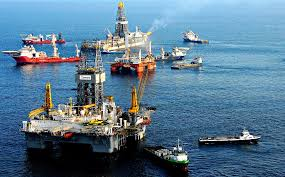
\includegraphics{osvbig}
	\caption{Offshore supply vessels in operation}
	\label{fig:shipforces}
\end{figure}
This requirement led to the development and subsequent popularity of dynamic position systems. Dynamic positioning (DP) is a computer-controlled system that maintains position and heading of a vessel automatically by using its propellers and thrusters. Information from position reference sensors that provide the vessel’s position and heading, along with information from wind sensors, motion sensors and gyrocompasses on the vessel are used by the system. The information is supplied as input to a program that calculates the changes in position/heading required to bring the vessel a preset location and, activates the vessel’s thrusters as necessary.

\begin{figure}
	\centering
	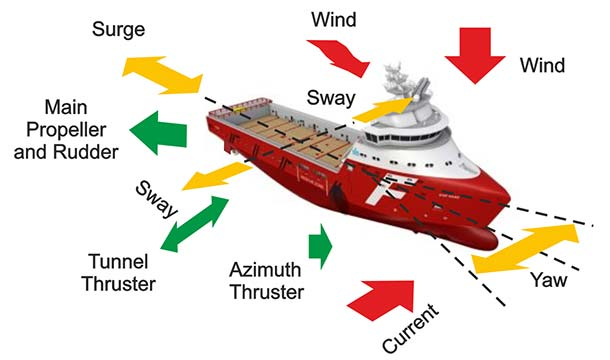
\includegraphics[scale=0.60]{dynamic-positioning}
	\caption{Forces acting on a ship and its possible movements}
	\label{fig:shipforces}
\end{figure}
\missingfigure{Make a sketch of the forces on a ship and its movements}
\todo[inline]{make own picture with legend of forces}
%Write about the popularity of Dp systems, its advantages and disadvantages. Mention increasing automation and the need for manual control ability. 

The use of dp systems has been increasing over the years since its first inception in 1960s. There are well over 2000 DP vessels in operation today \citep{sorensen2011survey}. From the early days of the technology where main focus areas of research were accurate position measurement and control system technologies used, research has now moved on to more specialized problems such as optimizing dp systems for energy efficiency. With increasing popularity of dp systems and increased use of sophisticated technology onboard ships, the marine industry can expect more advanced automation in vessel control over the years. Future systems could be enabled with features such as automatic maneuvering in shallow water and harbor areas, formation sailing, and automatic collision avoidance.

%The popularity of DP systems has grown to a point where they are a component of medium to large sized vessels these days. 

%This evolution of navigation technology on ships from mere position monitoring systems to automatic position control system has been accompanied by a corresponding growth of specialized personnel responsible for the monitoring of DP systems. 

%From PID to Advanced Control The first DP systems introduced in the early 1960s used conventional PID controllers in cascade with low-pass and/or notch filters to suppress the first-order wave-induced motion components. From the mid-1970s, more advanced control techniques were proposed based on linear optimal control and Kalman filter theory. With improvements and increasing sophistication in vessel control, the marine industry can look forward to more advanced control features such as DP-assisted position mooring systems, automatic maneuvering in shallow water and harbor areas, formation sailing, and automatic collision avoidance. These applications open new possibilities for the expansion of functionality in DP systems.




